\level{2}{Applicazione Android}
    Il diagramma sottostante rappresenta la vista ad alto livello dell'applicazione Android.
   
    \begin{figure}[H]\centering
        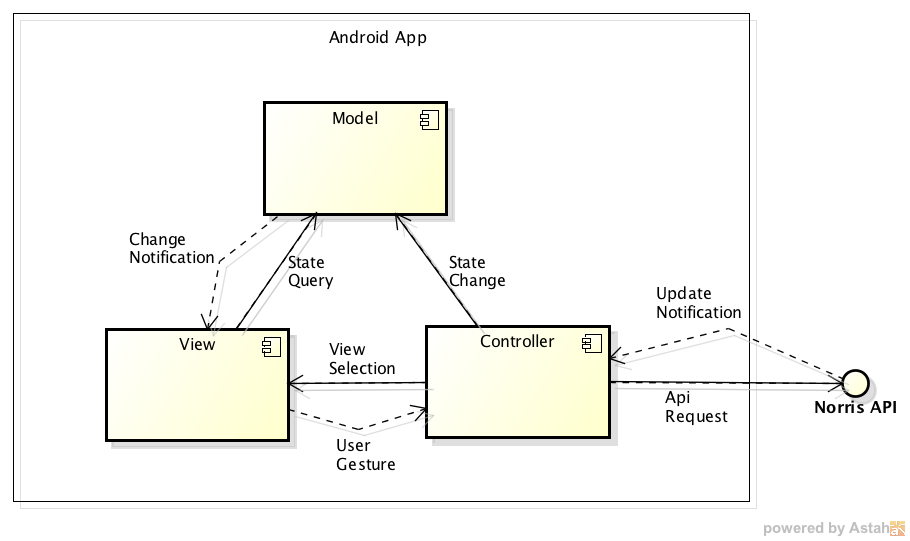
\includegraphics[width=\textwidth]{SpecificaTecnica/Pics/AndroidAppComponentDiagramLevel0.png}
        \caption{Diagramma delle componenti App Android}
    \end{figure}

    \level{3}{Descrizione delle componenti principali della app}
    	\level{4}{Model} 
        Il Model è la componente che rappresenta l'astrazione dei grafici visualizzati nell'applicazione. In essa sono contenuti i dati riguardanti i grafici, assieme alle relative impostazioni. In particolare sono presenti i modelli di tutte le tipologie di chart implementati da Norris. Il Data Model fornisce per ciascuna tipologia di grafico i metodi per inserire i dati e configurare alcune impostazioni. 
    
       \level{4}{View}
        La View è il componente che rappresenta le varie UI dell'applicazione e i vari widget dei grafici da inserire nelle UI. In tale componente potrebbero esser sollevati degli eventi scatenati dall'utente.
       \level{4}{Controller}
        Questo componente ha il compito di gestire tutto il controllo dell'applicazione. Le operazioni che esso gestisce sono riassunte nel seguente elenco:
        	\begin{itemize}
        		\item creazione del modello qualora questo sia necessario;
        		\item utilizzo delle API esterne di Norris;
        		\item interpretazione dei pacchetti ricevuti dal server contenenti i dati delle richieste API;
        		\item ascolto sul canale socket per ricevere gli aggiornamenti di stato dei chart;
        		\item interpretazione dei pacchetti di aggiornamento;
        		\item richiesta al modello di aggiornare il proprio stato;
        		\item richiesta della creazione dei widget dei grafici da inserire nelle UI dell'applicazioe;
        		\item avvio delle varie activity dell'applicazione;
        		\item gestione delle gesture dell'utente.
        \end{itemize}
    \level{3}{Descrizione delle interazioni che i componenti dell'app hanno tra di loro}
    	Le interazioni tra i componenti sono rappresentati con una freccia. Sono presenti due tipologie di frecce:
    	\begin{itemize}
    			\item{continua: } rappresenta l'invocazione di un metodo;
    			\item{tratteggiata: } rappresenta lo scatenarsi di un evento.
    		\end{itemize}
    	Riportiamo di seguito la descrizione di ogni interazione.
    	\level{4}{User Gesture}
	    La freccia etichettata con il termine "User Gesture" rappresenta l'interazione tra View e Controller. In seguito all'esecuzione di una gesture da parte dell'utente, la View notifica il Controller tramite l'emissione di un evento opportuno. Il Controller si occupa quindi di gestire tale evento. Questa interazione si verifica in particolare quando l'utente seleziona un item della lista dei grafici presenti nell'istanza di Norris richiesta.
	    \level{4}{API Request}
	    La freccia etichettata con il termine "API Request" rappresenta l'interazione tra il Controller e le API esterne di Norris. Il Controller richiama le API esterne per connettersi ad un'istaza di Norris, per richiedere la lista di grafici presenti presso quell'istanza e per ottenere le informazioni sui singoli grafici. Le API esterne rispondono al Controller con l'invio dei dati richiesti solo se l'autenticazione è andata a buon fine. Per la spiegazione in dettaglio delle funzionalità offerte dalle API esterne, si rimanda al documento \insdoc{Analisi dei Requisiti v.X.xx}.
	    \level{4}{Update Notification}
	   	La freccia etichettata con il termine "Update Notification" rappresenta l'interazione tra le API esterne di Norris e il Controller. Le API esterne notificano il Controller che è stato aggiornato il modello di un grafico nel Server. Tramite il canale socket viene inviato l'aggiornamento avvenuto e l'id del grafico che è stato aggiornato, in modo che il Controller possa occuparsi della gestione dell'aggiornamento nell'applicazione.
	    	
	    \level{4}{State Change}
	    La freccia etichettata con il termine "State Change" rappresenta l'interazione tra il Controller e il Model. Il Controller richiede al Model di modificare il proprio stato in seguito alla richiesta di un nuovo grafico o in seguito all'aggiornamento di un grafico già presente.
	    \level{4}{Change Notification}
	   	La freccia etichettata con il termine "Change Notification" rappresenta l'interazione tra il Model e la View. Il Model notifica le View che lo osservano ogniqualvolta il suo stato viene modificato. Le View dovranno quindi modificare a loro volta il proprio stato, in modo da essere sempre coerenti col modello.
	    \level{4}{State Query}
	   	La freccia etichettata con il termine "State Query" rappresenta l'interazione tra la View e il Model. Questa interazione rappresenta la richiesta dello stato del Model da parte della View. Viene effettuata quando la View ha la necessità di esporre i dati del Model o qualcosa che sia dipendente dallo stato di quest'ultimo. Ciò si verifica quando si deve mostrare un nuovo grafico o quando si devono mostrare gli aggiornamenti di un grafico già presente.
	    \level{4}{View Selection}
	   	La freccia etichettata con il termine "View Selection" rappresenta l'interazione tra il Controller e la View. Tale interazione rappresenta la richiesta da parte del Controller di visualizzare una specifica Activity.

